\section{Configurazione Hardware}
\labelsec{Hardware Configuration}

Dopo aver procurato tutto il materiale utile all'implementazione fisica del progetto è necessario collegare tutto l'hardware in maniera corretta.

In questa fase è molto importante conoscere le uscite dei sensori e ogni singolo pin della Gpio del Raspberry. Per quanto riguarda i pin dei sensori, solitamente la loro funzione è riportata direttamente nel dispositivo. Per quanto riguarda la Gpio del raspberry è bene aver sotto mano lo schema corrispondente che riporta ogni singola funzione di ciascun pin.


\subsection{Schema di collegamento}

IMPORTANTE: Quando si procede a collegare i sensori al Raspberry è bene assicurarsi che i pin utilizzati siano corretti, soprattutto per quanto riguarda quelli di alimentazione (5v o 3,3v) in quanto uno sbagliato uso di essi può compromettere in maniera permanente il sensore.

\begin{figure}
	\centering
	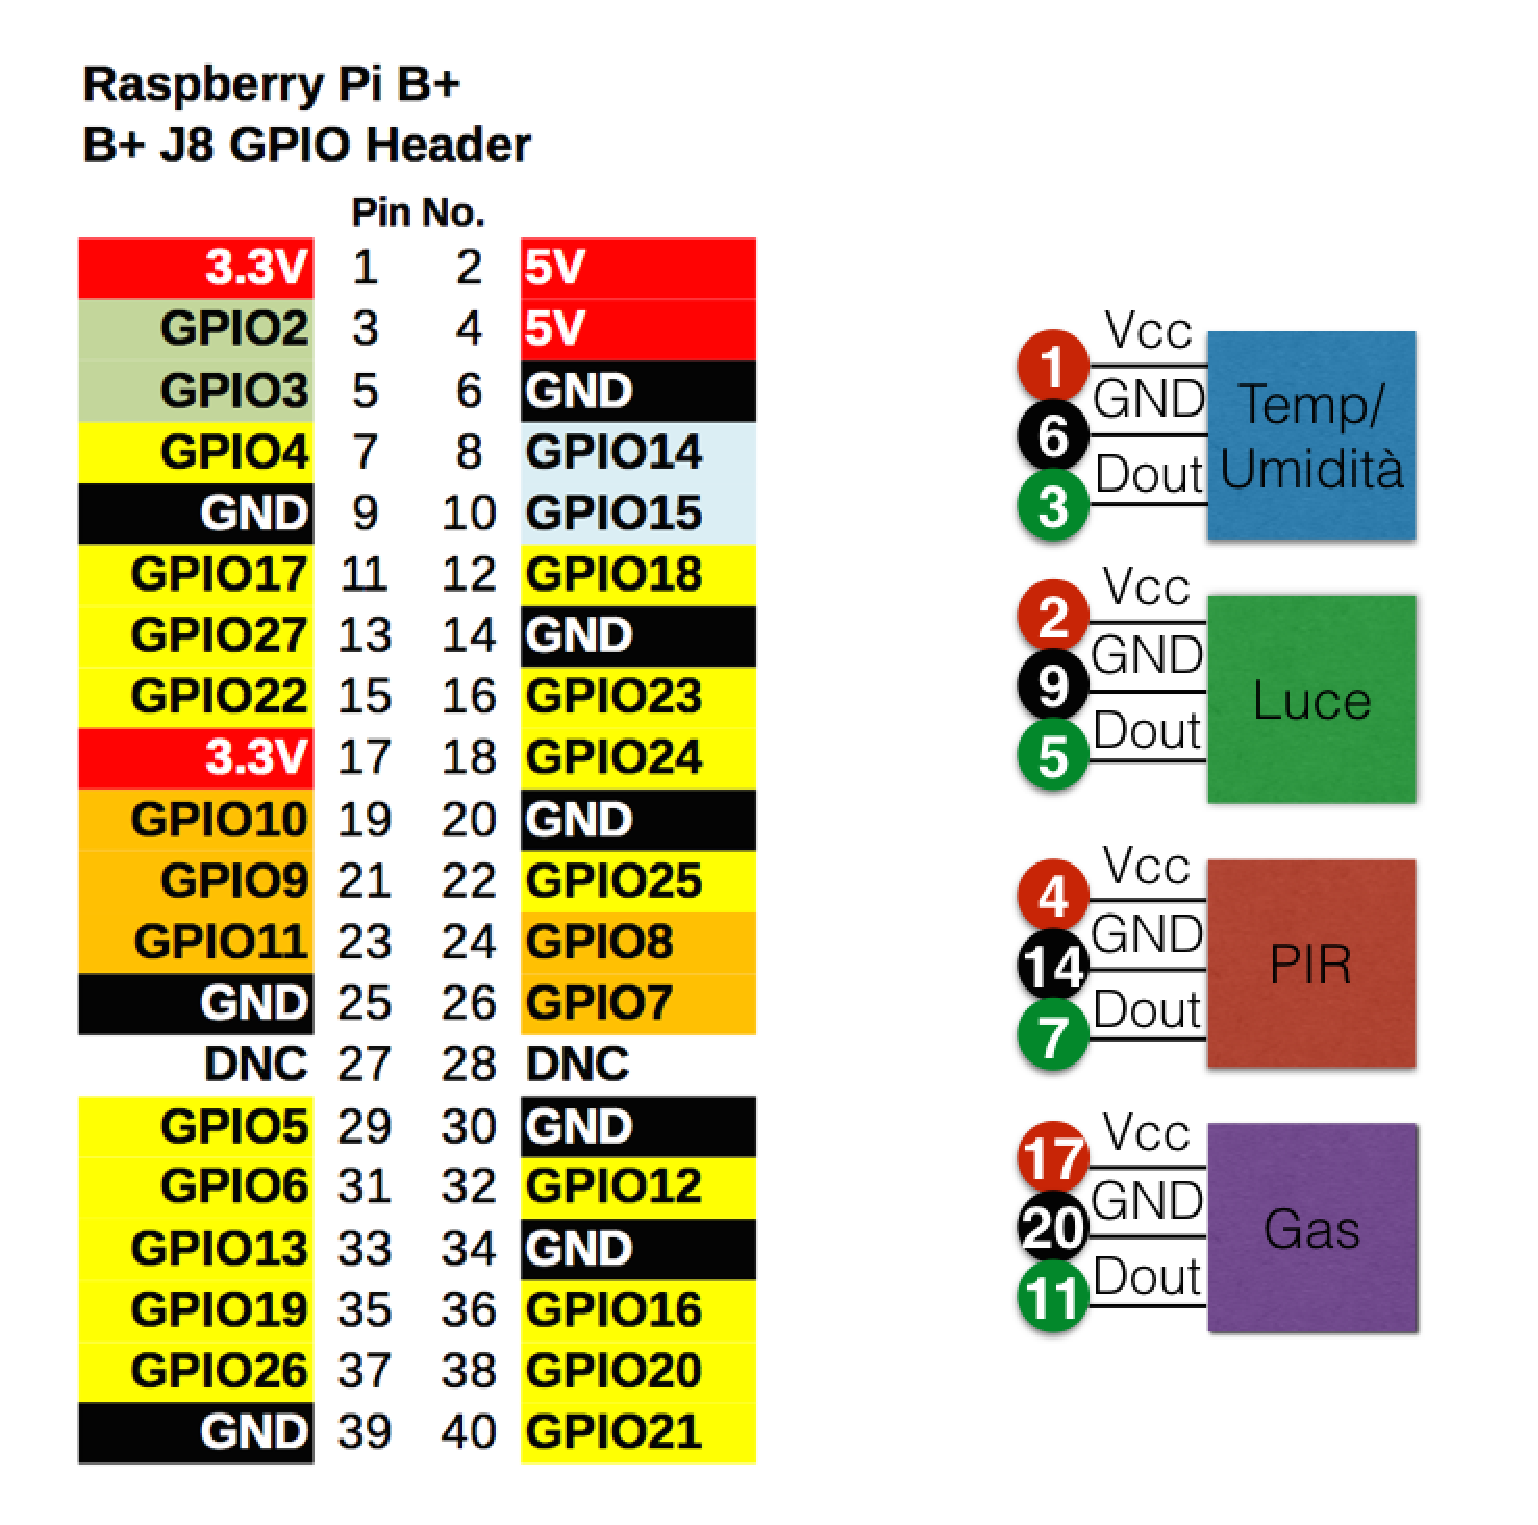
\includegraphics[width=0.7\linewidth]{Figures/Sensors&Rasp/hardwareconfig}
	\caption[confighardware]{Schema di collegamento}
	\label{fig:config}
\end{figure}



Lo schema di collegamento (figura~\ref{fig:config}) mostra la Gpio del Raspberry e gli accoppiamenti utilizzati nei sensori. Qual'ora il progetto voglia essere esteso sarà necessario procurarsi una fonte di alimentazione esterna in quanto il Raspberry mette a disposizione solo quattro pin di alimentazione.

\newpage